\chapter{SQL Databáze a jejich princip}
SQL (Structured Query Language), jazyk pro získávání strukturovaných dat, vznikl z jazyka SEQUEL, který vynalezla společnost IBM v 70. letech minulého století jako jazyk sloužící z získání takzvaných relačně orientovaných dat. Inspirací byl jeden z prvních relačních modelů, zvaný "A Relational Model of Data for Large Shared Data Banks" \cite{coddSql}, jehož autorem je Edgar F. Codd.  Během let se relačně orientované databáze osvědčily a dnes jsou používány ve spoustě aplikací na celém světě. Pojem SQL se postupem času zažil jako pojmenování celého odvětví databázových serverů, postavených na stejném nebo velmi podobném principu relační správy dat.

SQL databáze jsou tedy typickém zástupcem relačních databází, kde základním prvkem je tzv. relace. Můžeme je definovat podle Jaromíra Skřivana jako množinu tabulek, které se skládají ze sloupců a řádků. Sloupce odpovídají jednotlivým vlastnostem (atributům) entity. Údaje v jednom řádku tabulky reprezentují právě jednu entitu.
Budu mít např. tabulku ZAMĚSTNANEC, která bude popisovat entitu pracovníka ve firmě. Sloupce tabulky budou: ČÍSLO, JMÉNO, PŘÍJMENÍ, DAT\_NAR, PLAT a SMLOUVA\_OD. Atribut DAT\_NAR značí datum narození pracovníka a SMLOUVA\_OD uvádí datum, od kterého je pracovník v naší firmě zaměstnán \cite{sqlDatabaze}. Představme si, že reálnému světu odpovídá následující naplnění tabulky.

\begin{figure}[h]
\begin{centering}
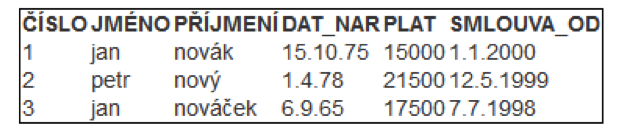
\includegraphics[scale=1]{obrazky/sql-tabulka}
\par\end{centering}
\caption{SQL Tabulka \cite{sqlDatabaze} \label{fig:sqlTable}}
\end{figure}


Data jsou tedy v databázi uspořádána do tabulek, kde každá tabulka má přesně daný počet sloupců, tabulka je tedy modelem uložení dat. 
K obsluze SQL databáze se používá speciální dotazovací jazyk SQL, který se podle Skřivana skládá z několika částí:
\begin{itemize}
\item Data Definition Language (DDL)
\item Storage Definition Language (SDL)
\item View Definition Language (VDL)
\item Data Manipulation Langugage (DML)
\end{itemize}
První částí jazyka SQL je jazyk DDL. Jedná se o jazyk pro vytváření databázových schémat a katalogů. Způsob ukládání dat v tabulkách definuje jazyk SDL. Třetí částí určenou pro návrhnáře a správce databází je jazyk VDL, který definuje databázové pohledy. Poslední částí je DML, jazyk popisující manipulaci s daty. Jeho součástí jsou známe příkazy INSERT, UPDATE, DELETE a nejpoužívanější příkaz SELECT \cite{sqlDatabaze}.

Relační SQL databáze jsou schopny pokrýt všechny typy vazeb, včetně vazby m:n, kterou je ale nutné implementovat pomocí vazebních tabulek \footnote{Tabulky nesoucí dvojice unikátních identifikátorů reprezentující relaci mezi dvěma entitami.}. Zároveň tyto databáze plně podporují cizí klíče. Mezi nejznámější SQL databázové servery patří MySQL, MSSQL, PosgreSQL nebo Oracle. MySQL je open source databázový server vyvinutý firmou Sun, dnes patřící společnosti Oracle. Tento databázový server je dostupný zdarma a je velmi oblíbený mezi vývojáři PHP webových aplikací. MSSQL je implementace SQL serveru od společnosti Microsoft, často používaná mezi vývojaři ASPX aplikací.
Většina z nich podporuje primární i sekundární indexování atributů, tedy je čistě na programátorovi nebo návrháři databáze, aby navrhl atributy, které bude vhodné indexovat a zrychlit tak odezvu databáze. Postupem času se tyto databáze vyvinuly a dnes nabízejí také možnosti pro ukládání souborů nebo geometrických dat.

\section{Princip ukládání dat}
SQL databáze typicky ukládají data do tabulek, které představují schéma (model) entit, v nich uložených. Jednotlivé atributy entity reprezentují sloupce tabulky, mají určitý datový typ například celé číslo, časový údaj nebo řetězec. Každému sloupci lze definovat jeho délku, což umožňuje velmi dobře omezit podobu ukládáných dat a zároveň šetřit diskový prostor databázového serveru. Některým sloupcům mohou být nastaveny výchozí hodnoty nebo být označeny jako nepovinné. Každý sloupec určený pro atribut typu řetězec, musí být nastavené kódování. Nepsaným standardem je pro tyto atributy používat UTF-8. \footnote{Způsob kódování řetězců podporující veškeré znaky národních abeced Unicode.} Jeden ze sloupců (zpravidla první), by měl být označen jako takzvaný \emph{primární klíč}. V tomto sloupci musí být uložen unikátní identifikátor řádku tabulky a databázový server poté sám kontroluje jedinečnost tohoto sloupce. Primární klíč může obsahovat uměle vytvořenou nebo přirozeně se vyskytující jedinečnou hodnotu, například rodné číslo. Struktura SQL tabulky je tedy předem daná a každá změna v ní musí být aplikována na všechny řádky, které obsahuje. To v praxi znamená, že přidání nebo odebrání sloupce v tabulce obsahující velké množství záznamů, představuje časově velice náročnou operaci \cite{mysqlDataTypes}.
Většina v současnosti používaných databázových serverů dobře podporuje indexování atributů, které primárně slouží k urychlení dotazování na tabulku. Index by měl být přidán na ty sloupce, u kterých se očekává časté použití v SQL dotazech. Indexy mohou být také použity k ověření jedinečnosti dat ve sloupci (tzv. unikátní index) nebo pro fulltextové vyhledávání.

\begin{figure}[h]
\begin{centering}
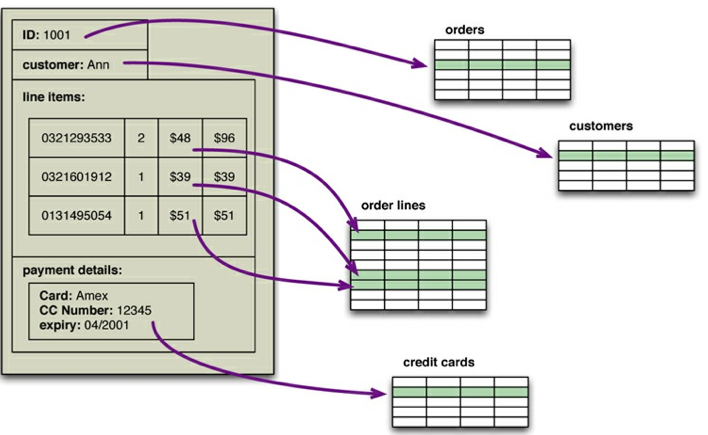
\includegraphics[scale=0.5]{obrazky/data2table}
\par\end{centering}
\caption{Ilustrace webového formuláře a potřebých datulek s daty \cite{nosqlDistilled} \label{fig:data2table}}
\end{figure}

Z principu relačních databází vyplývá, že pro zachycení složitějších vazeb nebo hierarchických dat je nutné použít velké množství tabulek. Vztah mezi zobrazením a reprezentací dat dobře ilustruje obrázek výše, jednoduché vztahy mezi objednávkou (tabulka orders) a zákazníkem (tabulka customers) jsou realizovány pomocí cizích klíčů. Na složitější vazby typu m:n je třeba vytvořit nové vazební tabulky (order lines), které slouží pouze tomuto účelu a nenesou žádná další data.

\vspace{0.5cm}
\noindent \emph{Některé datové typy v MySQL}
\begin{itemize}
\item INT, INTEGER - celé číslo, rozsah cca -2 až 2 milióny, existují varianty s větším rozsahem hodnot
\item FLOAT, DOUBLE - desetinné číslo
\item DATE, DATETIME, TIMESTAMP - reprezentace času
\item CHAR, VARCHAR, TEXT - řetězce
\item BLOB - binární data
\end{itemize}

\section{Integrita dat v SQL databázích}
Většina SQL serverů poskytuje záruky integrity dat, databázové operace se zpravidla provádějí v transakcích, které musí splňovat tzv. \emph{vlastnosti ACID} \cite{acid}.
\begin{itemize}
\item Atomic (atomičnost) - každá transakce musí být atomická, provedou se buď všechny změny v databází nebo žádná
\item Consistent (konzistence) - transakce představuje přechod z jednoho konzistentního stavu databáze do druhého
\item Isolated (izolace) - každá transakce je nezávislá a nemůže být ovlivněna ostatními transakcemi
\item Durable (trvanlivost) - pokud je transakce dokončena, změny, které provedla, jsou trvalé
\end{itemize}
Každá transakce představuje operaci provedenou uživatelem aplikace, tedy například objednávku z internetového obchodu nebo finanční operaci pracovníka pobočky v bankovním systému. Obsahuje všechny změny v tabulkách, které jsou pro daný úkon vzhledem k návrhu aplikace potřeba. Transakce fungují jako mechanismus ochrany před nekonzistencí databáze, poskytují záruky, že nedošlo k ztrátě nebo poškození vstupních dat a že všechny změny v tabulkách proběhly úspěšně. Transakce se v databázových systémech zahajují příkazem \emph{BEGIN}, po němž následují operace s databází. Pokud nedojde k chybě v některé z nich, je transakce dokončena příkazem \emph{COMMIT}. V opačném případě se pomocí příkazu \emph{ROLLBACK} databáze vrátí do konzistentního stavu před zahájením transakce \cite{transactions}.

Existují dva přístupy k vnitřnímu zpracování transakcí databázovým serverem. První z nich, zvaný optimistický, předpokládá úspěch celé transakce a zapisuje změny rovnou do tabulek, do něchž pak v případě neúspěchu celé transakce opět zapíše původně uložená data. Druhý přístup, zvaný pesimistický, ukládá data do dočasného úložiště, ze kterého je pak v případě úspěchu transakce zapíše do databázových tabulek. Hlavní výhodou pesimistického přístupu je fakt, že server nepracuje s uloženými reálnými daty v průběhu transakce. Tento přístup ale vykazuje nižší rychlost zpracování kvůli vyšším nárokům na systémové prostředky a paměť serveru. Každé aktuálně prováděné transakci totiž musí být přidělen prostor v paměti. Naproti tomu optimistický přístup nabízí velmi vysokou rychlost zpracování úspěšně provedených transakcí, zatímco v případě chyby je rychlost zotavení databáze velmi nízká \cite{pesimistic_optimistic}.

\begin{figure}[h]
\begin{centering}
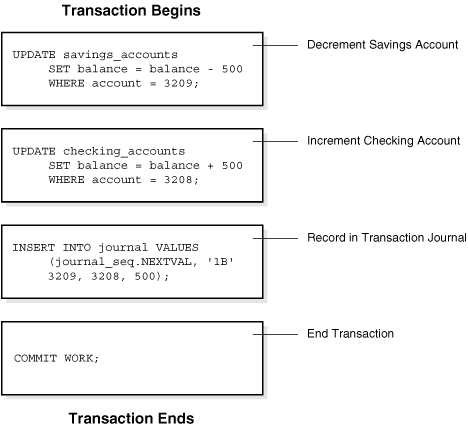
\includegraphics[scale=0.5]{obrazky/sql_transakce}
\par\end{centering}
\caption{Databázová transakce \cite{oracle_transactions} \label{fig:oracleTransactions}}
\end{figure}

\pagebreak
\section{Možnosti replikace a škálovatelnosti}
Při návrhu většiny dnes používaných SQL databázových serverů nebyla brána v úvahu dobrá podpora škálovatelnosti,  možnosti běhu v tzv. \emph{distribuovaném prostředí} tedy na několika serverech zároveň. V dobách jejich vývoje byl totiž Internet značně odlišný o toho jaký známe dnes, neexistovali tak obrovská datová úložiště s nutností rychlého a paralelního přístupu. V dnešní době všechny majoritní SQL servery podporují replikaci a společně s load balancerem \footnote{Server, který shromažďuje požadavky na databázi a rozděluje je rovnoměrně mezi všechny připojené databázové servery.} lze také dosáhnout velmi vysokého výkonu. Sofistikovaným řešením je například technologie MySQL Galera Cluster, která umožňuje provozovat plnohodnotný databázový cluster i s klasickou relační databází MySQL. Data mezi jednotlivými servery jsou transakčně replikovány, zátěž rozděluje vestavěný load balancer. Tato technologie také částečně umožňuje horizontální škálování přidáním serverů, podobné tomu, kterým disponují nové NoSQL databáze  \cite{galeracluster}.